\clearpage
\phantomsection

\setcounter{chapter}{4}

\chapter[{THỰC THI VÀ ĐÁNH GIÁ}]{thực thi và đánh giá}
Chương 5 sẽ mô tả về quá trình thực thi và kiểm thử thực tế với một hệ thống System on Chip để đánh giá về hiệu năng, đồng thời chứng minh IP đã thiết kế đảm bảo khả năng hoạt động với các thành phần khác.
\section{Thông tin về bo mạch Zynq UltraScale+MPSoC ZCU106 Evaluation Kit}
ZCU106 Evaluation Kit là bo mạch được phát triển để phục vụ mục đích thiết kế và tạo mẫu các hệ thống nhúng trên nền tảng của nhà sản xuất Xilinx. Nó là tổ hợp của hai phần gồm hệ thống xử lý (PS) và FPGA (PL). Với PL là hệ logic khả trình cho phép người dùng lập trình phần cứng để thực hiện các chức năng chuyên biệt với công nghệ 16nm FinFET+. PS là ARM flagship Cortex-A53 64-bit quad-core processor và Cortex-R5F dual-core real-time processor. Ngoài ra trên bo mạch còn tích hợp rất nhiều các ngoại vi như HDMI, Ethernet, ...
\begin{figure}[!ht]
	\centering
	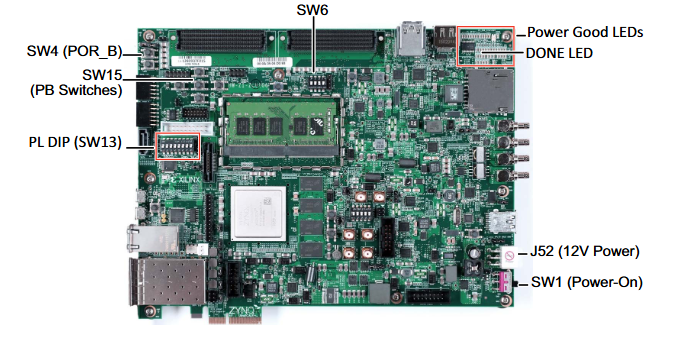
\includegraphics[width=1\linewidth]{figures/zcu106.png}
	\caption{Bo mạch ZCU106 UltraScale+MPSoC}
	\label{fig:zcu106}
\end{figure}
\section{Xây dựng hệ thống SoC}
Sau khi đã có những thiết kế RTL, cần đóng gói thiết kế thành IP. IP sẽ sử dụng các giao tiếp theo chuẩn giao tiếp AXI4-Stream. Giao diện của IP được mô tả tại hình \ref{fig:ipInterface}
Hình \ref{fig:soc1} mô tả về sơ đồ khối của hệ thống SoC sẽ được xây dựng. Ảnh có thể được lưu trữ trong DDR, sau đó DMA sẽ lấy dữ liệu ảnh trong DDR đó, chuyển vào khối IP. Vì có tín hiệu \textbf{start} để yêu cầu việc bắt đầu quá trình nên sẽ có một khối GPIO được điều khiển bởi PS để thực hiện bật, tắt chân start. Từ IP, một tín hiệu ngắt cũng sẽ được nối trở về PS để thực hiện thông báo ngắt khi cần. 
\begin{figure}[H]
	\centering
	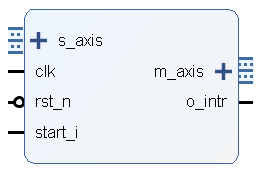
\includegraphics[width=0.8\linewidth]{figures/ipInterface.png}
	\caption{Giao diện của IP MRELBP}
	\label{fig:ipInterface}
\end{figure}
\begin{figure}[!ht]
	\centering
	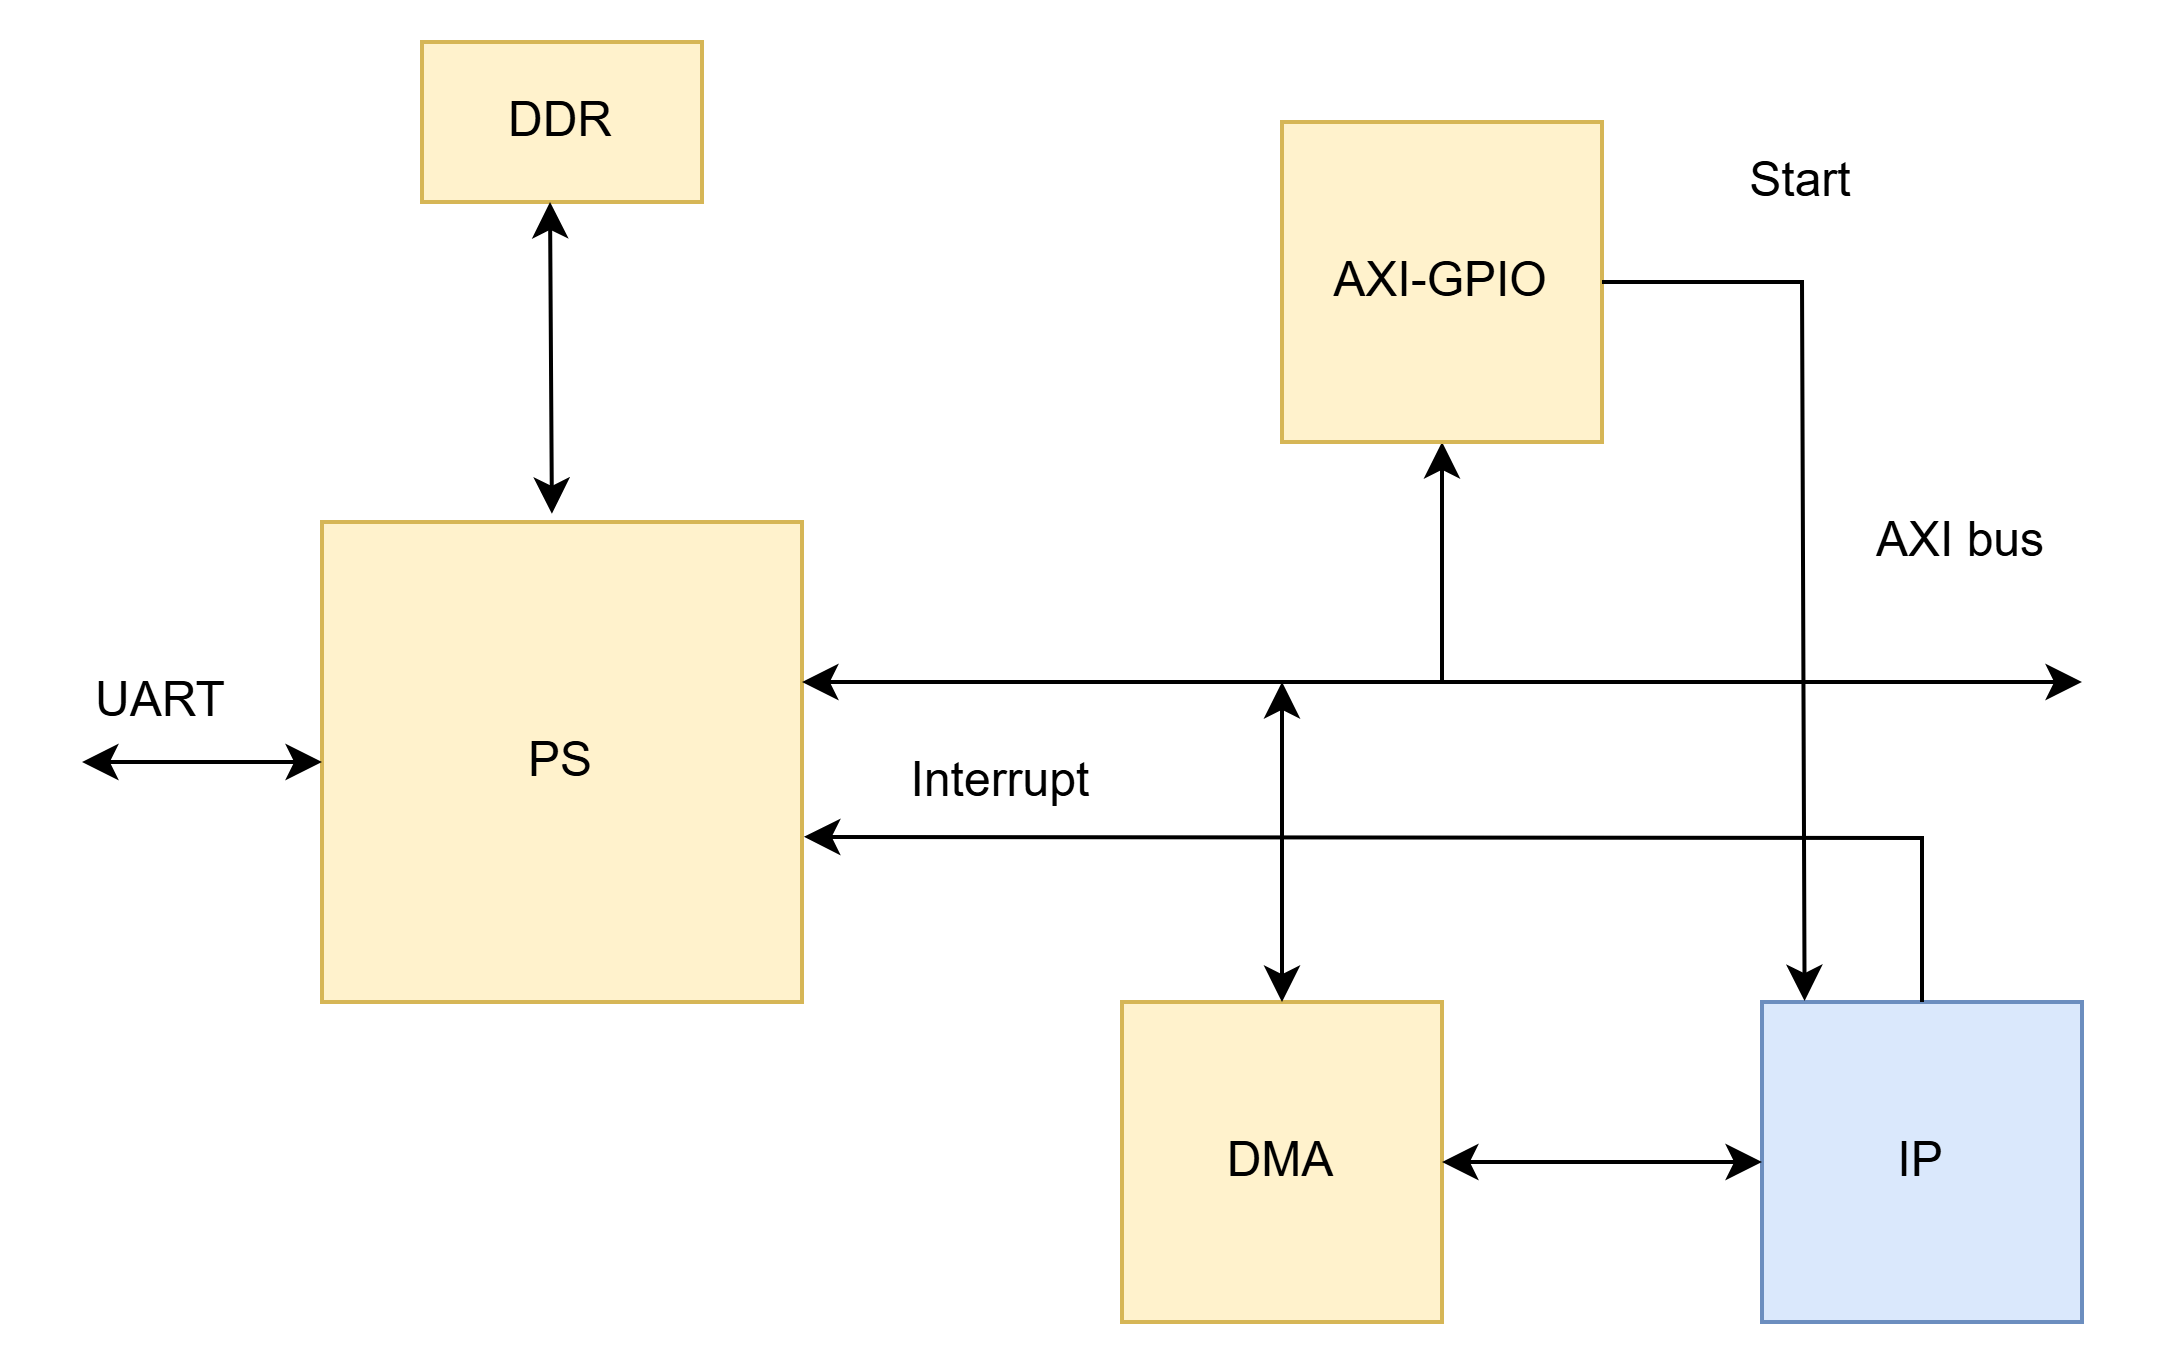
\includegraphics[width=0.8\linewidth]{figures/soc1.png}
	\caption{Sơ đồ khối hệ thống SoC}
	\label{fig:soc1}
\end{figure}
\begin{figure}[!ht]
	\centering
	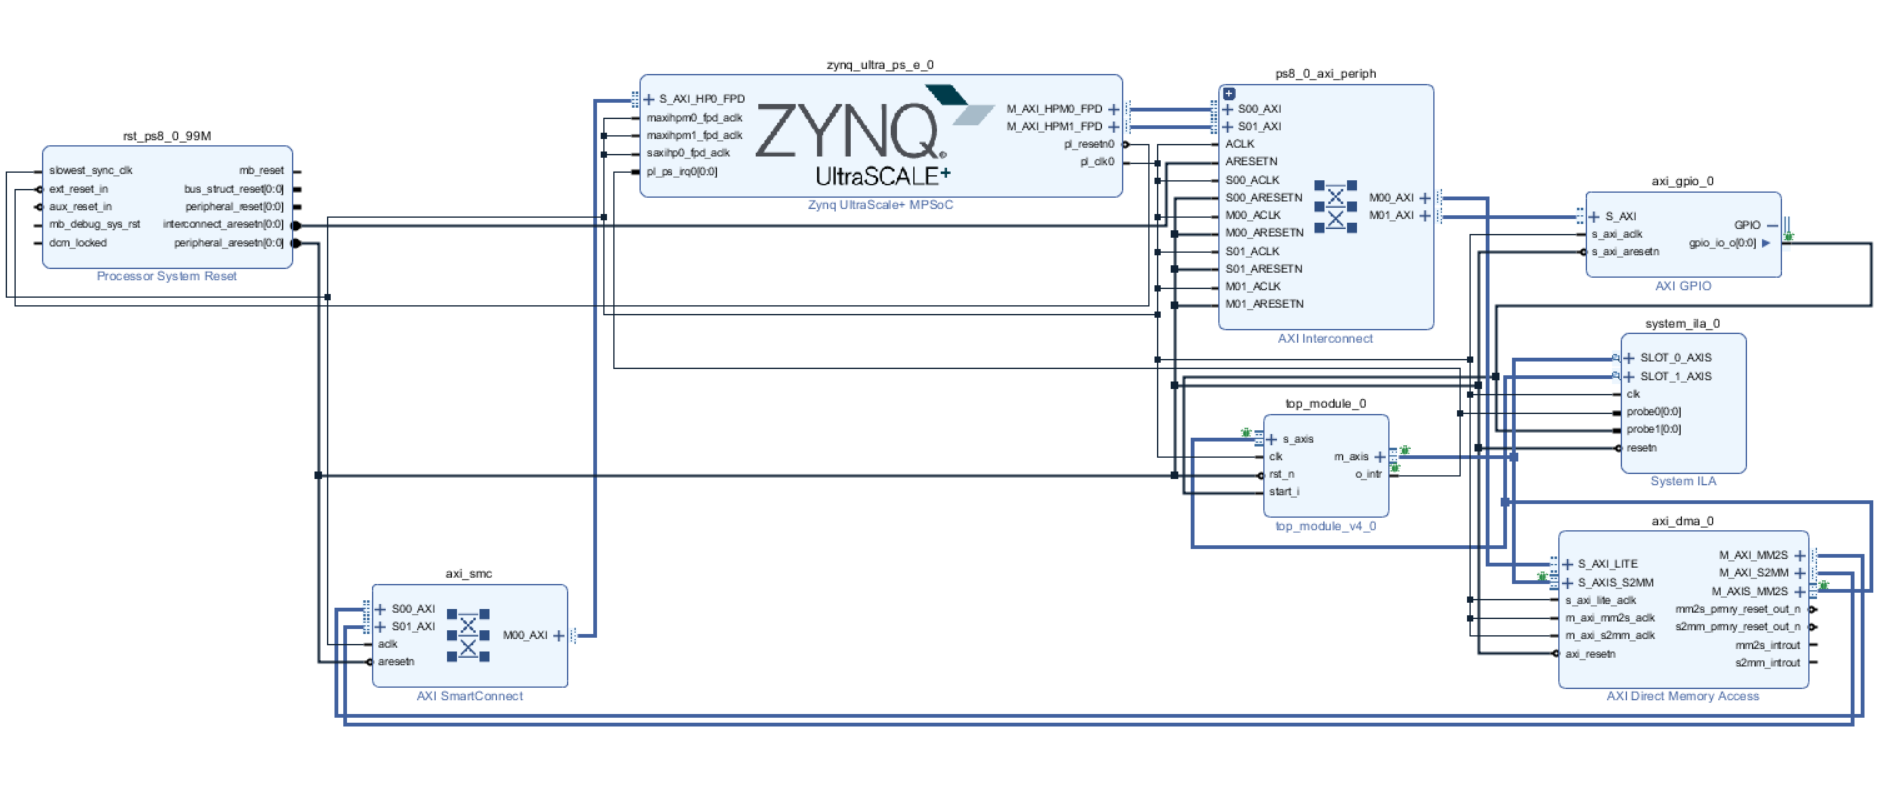
\includegraphics[width=\linewidth]{figures/socreal.png}
	\caption{Thiết kế khối hệ thống SoC}
	\label{fig:socreal}
\end{figure}
\begin{figure}[H]
	\centering
	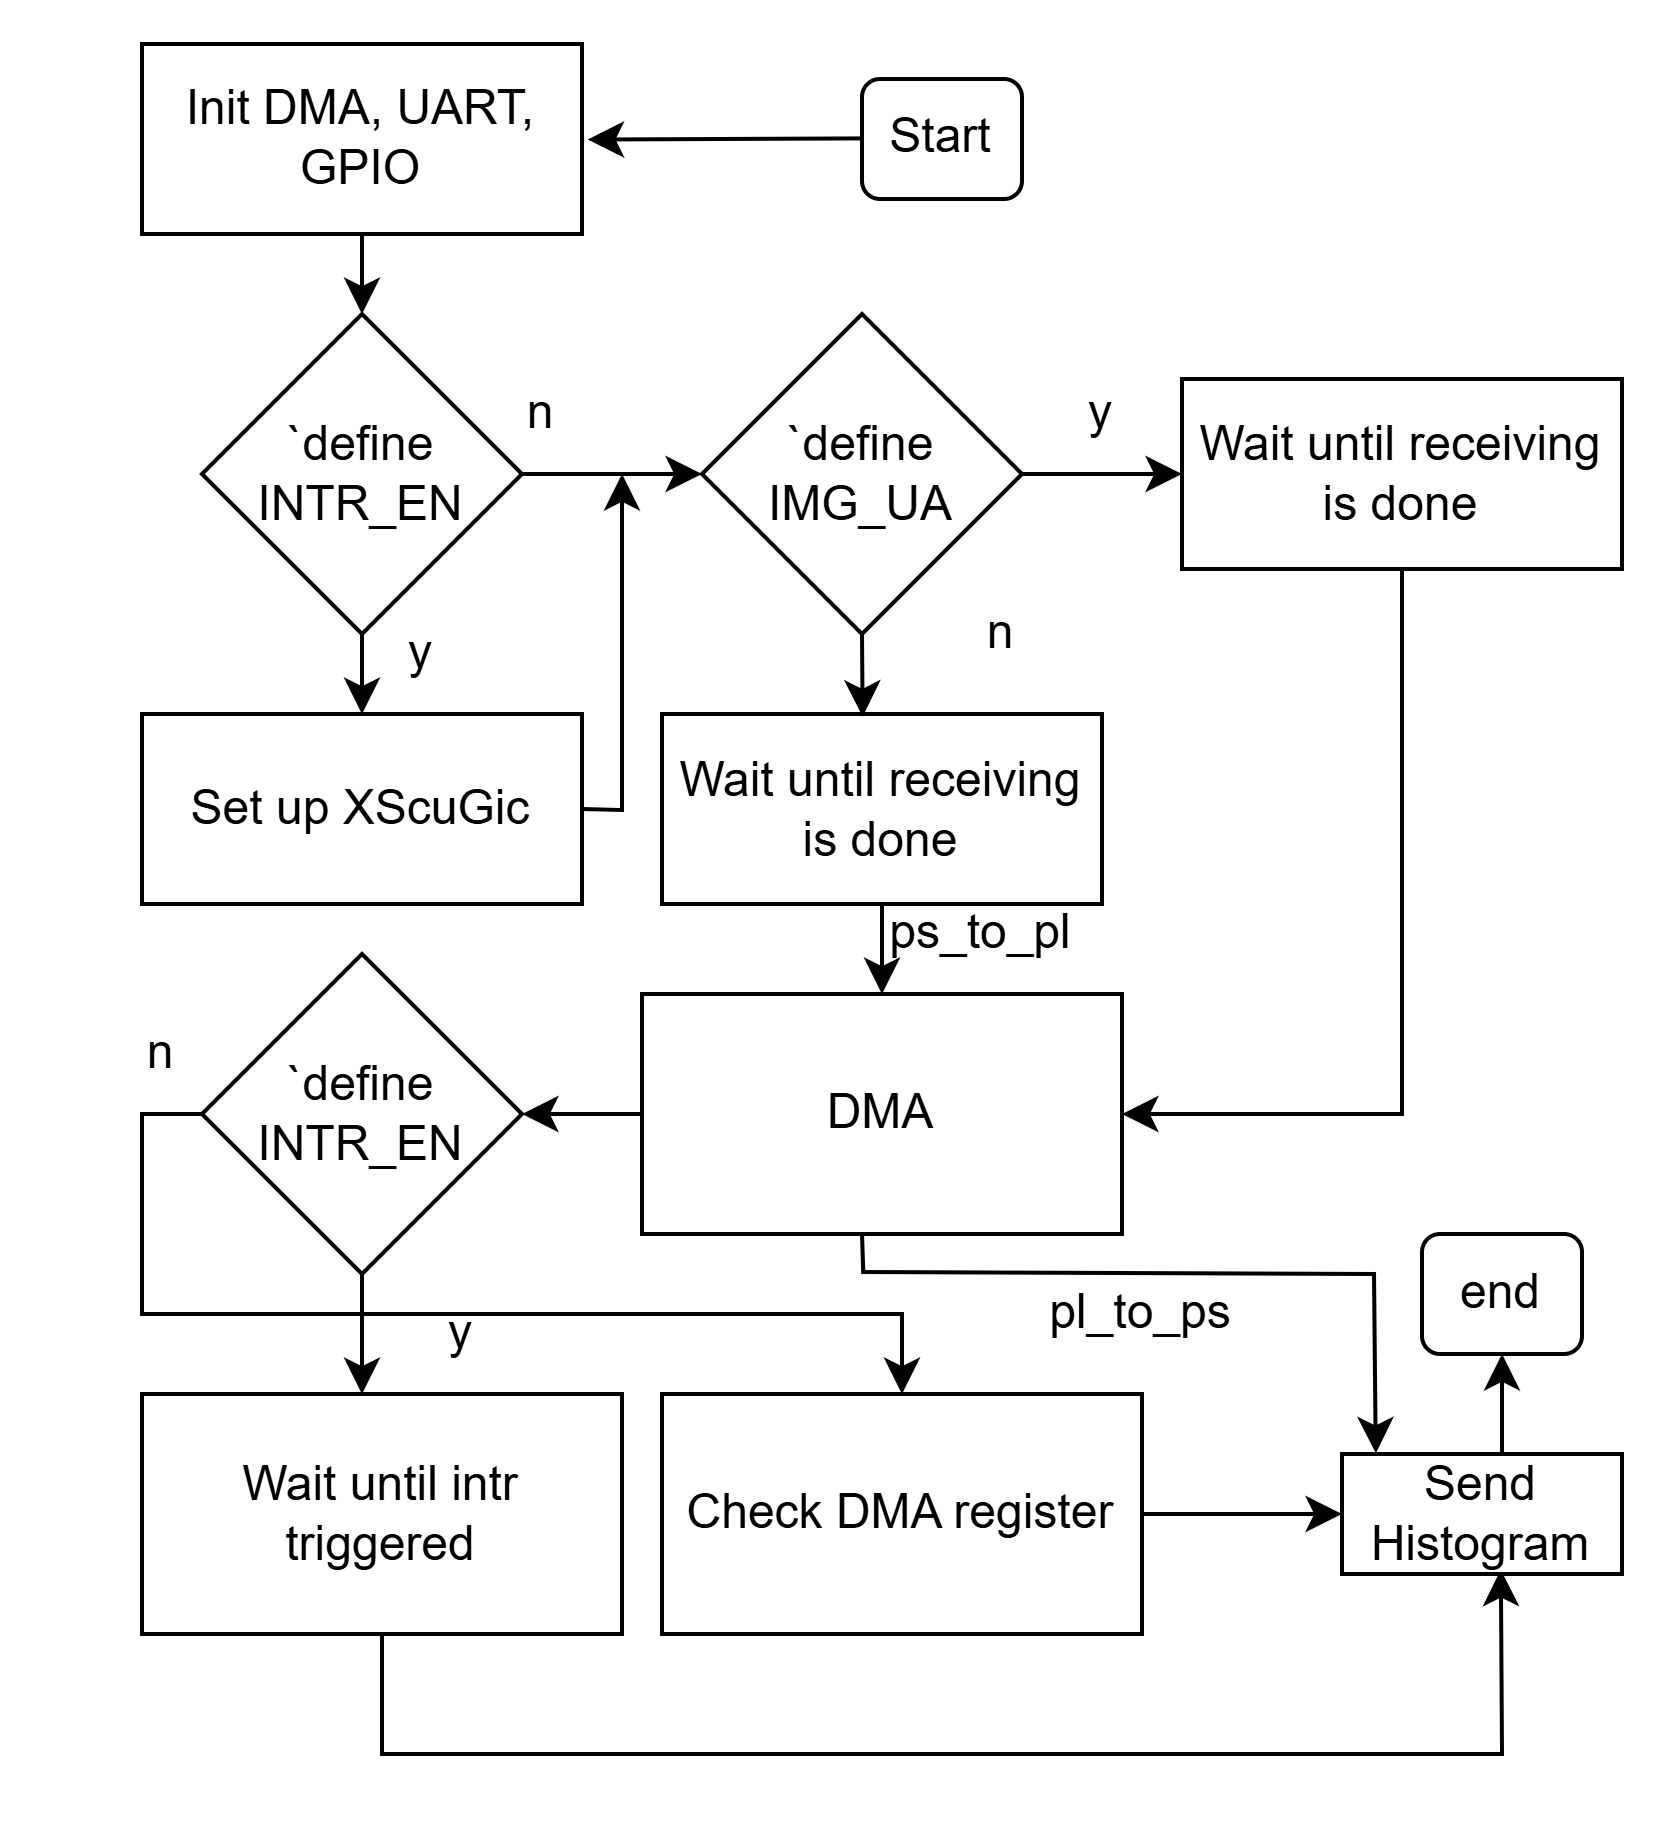
\includegraphics[width=0.8\linewidth]{figures/socflow.png}
	\caption{Lưu đồ hoạt động của chương trình phần mềm}
	\label{fig:socflow}
\end{figure}
Hình \ref{fig:socflow} mô tả lưu đồ hoạt động của chương trình phần mềm cho hệ thống SoC đã thiết kế. Khi chương trình bắt đầu thì sẽ cần khởi tạo các khối cần sử dụng bao gồm DMA, UART và GPIO. Nếu định nghĩa một cờ là INTR\_EN thì sẽ cần thiết lập về mức ưu tiên ngắt và thời điểm kích hoạt ngắt. Nếu định nghĩa cờ IMG\_UA thì sẽ kích hoạt UART nhận dữ liệu từ bên ngoài, nếu không sẽ lấy được ảnh đã lưu trữ cục bộ, sau đó thông qua bộ DMA đưa dữ liệu vào IP đã thiết kế. Nếu định nghĩa cờ ngắt, quá trình đợi tính toán hoàn tất sẽ kết thúc khi mà ngắt được kích hoạt, nếu không sẽ cần kiểm tra các thanh ghi của DMA để xem DMA đã hoàn tất quá trình hoạt động hay chưa. Sau khi kết thúc có thể tiến hành gửi các giá trị đặc trưng qua kết nối UART để quan sát hoặc sử dụng cho mục đích khác.
\section{Kết quả và đánh giá}
Kết quả về tổng hợp và thực thi sẽ được thực hiện trên phần mềm Vivado. Kết quả tổng hợp bao gồm về tài nguyên sử dụng, tần số tối đa, năng lượng tiêu thụ. Để đánh giá về độ chính xác của mô hình sẽ thực hiện với tập dữ liệu Outex, so sánh thời gian thực tế với thời gian chạy của các mô hình phần mềm.

Tài nguyên sử dụng được mô tả trong bảng \ref{tab:resource}
\begin{figure}[!ht]
	\centering
	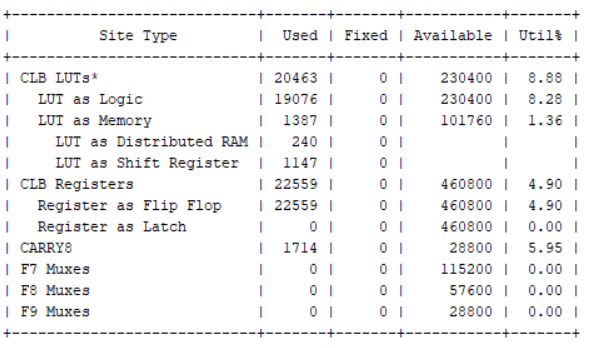
\includegraphics[width=\linewidth]{figures/synthesis_report.png}
	\caption{Báo cáo kết quả tổng hợp của phần mềm Vivado}
	\label{fig:synthesis_report}
\end{figure}
\begin{table}[H]
	\centering
	\renewcommand{\arraystretch}{1.3}
		\caption{Tài nguyên sử dụng}
	\begin{tabular}{|p{2cm} p{2cm} p{2cm} p{2cm} p{2cm} p{2cm}|}
		\hline
		\rowcolor{gray!30}
		\textbf{Tài nguyên} & \textbf{Sử dụng}  & \textbf{Có sẵn} & \textbf{Phần trăm} &  \textbf{Wang \cite{realTimeTexture}} & \textbf{HLS}  \\
		LUT & 20463 & 230400 & 8.88\% & 49033 & 30378
		\\ \hline
		FF & 22559 & 460800 & 4.9\% & 19969 & 13713
		\\ \hline
		BRAMs & 31.5 & 312 & 10.1\% & 41.5 & 88
		\\ \hline
	\end{tabular}

	\label{tab:resource}
\end{table}


Thông số định thời của hệ thống được thể hiện trên hình \ref{fig:ipTiming}. Với các thông số định thời ta sẽ có một số tiêu chí đánh giá như sau:
\begin{itemize}
	\item WNS: Đỗ trễ trong trường hợp xấu nhất của một xung nhịp, WNS = $min(T-T_n)$ với T là một chu kỳ của xung nhịp, $T_n$ là thời gian truyền. Để mạch hoạt động chính xác thì phải đảm bảo giá trị WNS lớn hơn 0.
	\item Tần số $F_{max}$: Tần số có thể chạy trên phần cứng trong một triển khai nhất định.
\end{itemize}
Hệ thống được xây dựng với ràng buộc đầu là 100MHz tương đương với chu kỳ xung nhịp là 10ns, từ đó ta có thể tính tần số tối đa như sau:
\begin{equation*}
	F_{max} = \frac{1}{T - WNS} = \frac{1}{(10 - 5.050)*10^{-9}} = 202   (MHz) 
\end{equation*}

\begin{figure}[!ht]
	\centering
	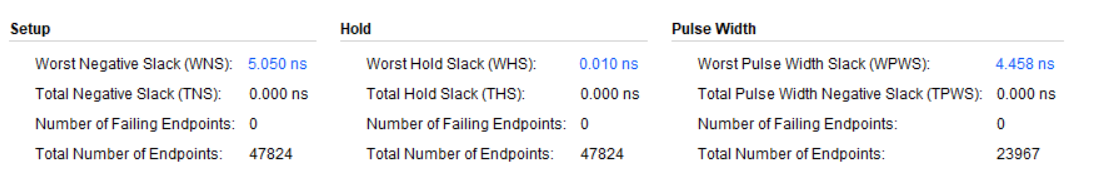
\includegraphics[width=\linewidth]{figures/ipTiming.png}
	\caption{Thông số định thời của thiết kế}
	\label{fig:ipTiming}
\end{figure}


Công suất tiêu thụ của hệ thống được thể hiện trong hình \ref{fig:power}. Công suất tiêu thụ của mạch khi hoạt động là 0.595 Watt. Đây là mức tiêu thụ năng lượng không quá lớn để tích hợp với các hệ thống khác vì hoạt động của IP rất phức tạp và cần tối ưu về mặt đáp ứng thời gian thực.

\begin{figure}[!ht]
	\centering
	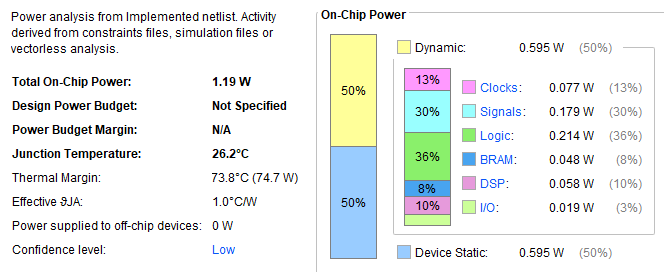
\includegraphics[width=\linewidth]{figures/power.png}
	\caption{Công suất tiêu thụ năng lượng của thiết kế}
	\label{fig:power}
\end{figure}

Để kiểm tra độ chính xác của thiết kế, ta sẽ đánh giá đặc trưng đã trích xuất với tập dữ liệu Outex\cite{outex} và các mô hình cổ điển. Dữ liệu từ tập dữ liệu Outex được xây dựng nhằm phát triển một bộ khung linh hoạt và cơ sở dữ liệu hình ảnh phục vụ cho việc đánh giá thực nghiệm các thuật toán phân tích kết cấu. Dữ liệu này bao gồm một tập hợp lớn các kết cấu bề mặt được thu thập dưới nhiều điều kiện khác nhau, giúp xây dựng nhiều bài toán phân tích kết cấu đa dạng. 4 mô hình học máy cổ điển được sử dụng là SVM (Support Vector Machine), Logistic Regression, Naive Bayes và KNN (K-Nearest Neighbor) với K bằng 3. 



\begin{table}[!ht]
	\centering
	\renewcommand{\arraystretch}{1.2}
		\caption{Độ chính xác trên các tập dữ liệu với SVM}
	\begin{tabular}{|p{2.5cm} p{2.5cm} p{2.5cm} p{2.5cm} p{2.5cm} p{2.5cm}|}
		\hline
		\rowcolor{gray!30}
		\textbf{Tập dữ liệu} & \textbf{MRELBP(1)}  & \textbf{MRELBP(2)} & \textbf{MRELBP(3) } &  \textbf{MRELBP(4)} & \textbf{MRELBP(5)}  \\
		TC\_00010\_r & 100 &98.75 & \textbf{99.79 }& 100 & 100
		\\ \hline
		TC\_00010\_c & 100 & 98.75 & \textbf{99.79} & 100 & 100
		\\ \hline
		TC\_00011\_r & 94.58 &92.5 & \textbf{93.5} & 94.58 & 92.29
		\\ \hline
		TC\_00012\_i & 99.58 & 97.58 & \textbf{98.54} & 99.58 & 97.92
		\\ \hline
		TC\_00020 & 99.17 & 97.5 & \textbf{99.17} & 99.17 & 99.58
		\\ \hline
		TC\_00023 & 97.92 &98.54 & \textbf{98.12} & 97.92 & 98.33
		\\ \hline
		TC\_00024 & 96.46 & 92.71 & \textbf{96.25} & 96.46 & 96.88
		\\ \hline
		TC\_00030 & 99.17 & 97.5 & \textbf{99.17} & 99.17 & 99.38
		\\ \hline
		TC\_00033 & 97.08 & 96.46 & \textbf{97.08} & 97.08 & 96.25
		\\ \hline
		TC\_00034 & 96.67 & 92.71 & \textbf{96.25} & 96.67 & 96.88
		\\ \hline
	\end{tabular}

	\label{tab:svm}
\end{table}

\begin{table}[!ht]
	\centering
	\renewcommand{\arraystretch}{1.3}
	\caption{Độ chính xác trên các tập dữ liệu với Logistic Regression}
	\begin{tabular}{|p{2.5cm} p{2.5cm} p{2.5cm} p{2.5cm} p{2.5cm} p{2.5cm}|}
		\hline
		\rowcolor{gray!30}
		\textbf{Tập dữ liệu} & \textbf{MRELBP(1)}  & \textbf{MRELBP(2)} & \textbf{MRELBP(3) } &  \textbf{MRELBP(4)} & \textbf{MRELBP(5)}  \\
		TC\_00010\_r & 99.58 & 99.92 & \textbf{100} & 99.58 & 100
		\\ \hline
		TC\_00010\_c & 99.58 &97.5 & \textbf{100} & 99.58 & 100
		\\ \hline
		TC\_00011\_r & 88.96 &91.46 & \textbf{93.75} & 88.96 & 93.13
		\\ \hline
		TC\_00012\_i & 95.21 &92.71 & \textbf{96.04} & 95.21 & 96.67
		\\ \hline
		TC\_00020 & 96.46 & 94.79 & \textbf{98.75} & 96.46 & 98.33
		\\ \hline
		TC\_00023 & 96.88 & 97.29 & \textbf{98.33} & 96.88 & 97.92
		\\ \hline
		TC\_00024 & 89.8 & 92.5 & \textbf{93.96} & 89.8 & 96.04
		\\ \hline
		TC\_00030 & 96.67 & 95.0 & \textbf{98.96} & 96.67 & 98.33
		\\ \hline
		TC\_00033 & 96.67 &96.25 & \textbf{98.33} & 96.67 & 97.29
		\\ \hline
		TC\_00034 & 86.88 & 91.88 & \textbf{95.42} & 86.88 & 95.63
		\\ \hline
	\end{tabular}
	
	\label{tab:lr}
\end{table}

Bảng \ref{tab:svm}, \ref{tab:lr}, \ref{tab:nb}, \ref{tab:knn} là kết quả đánh giá dựa trên tập huấn luyện Outex. Với MRELBP(1) là phiên bản với các giá trị bán kính là 2, 4, 6, thực hiện đúng các thao tác của công thức \ref{eq:relbp_ci}, \ref{eq:relbp_ni}, \ref{eq:relbp_rd}. MRELBP(2) với công thức CI theo \ref{eq:relbp_ci_op}. MRELBP(4) là phiên bản với các giá trị tính nội suy tham chiếu được cố định theo 24-bit trong đó 16-bit biểu diễn phần thập phân. Phiên bản MRELBP(3) là phiên bản với các giá trị tính nội suy cố định và CI tối ưu cho phần cứng. Phiên bản MRELBP(5) là phiên bản với các giá trị bán kính là 2, 4, 6, 8 với các giá trị tính nội suy cố định và CI tối ưu cho phần cứng. Kết quả đánh giá cho thấy, so với phiên bản cùng số lượng bán kính thì kết quả đạt được không có nhiều sự khác biệt, tương tự với phiên bản có thêm giá trị bán kính bằng 8 cũng cho thấy sự chênh lệch là rất ít. 

\begin{table}[!ht]
	\centering
	\renewcommand{\arraystretch}{1.3}
	\caption{Độ chính xác trên các tập dữ liệu với Naive Bayes}
	\begin{tabular}{|p{2.5cm} p{2.5cm} p{2.5cm} p{2.5cm} p{2.5cm} p{2.5cm}|}
		\hline
		\rowcolor{gray!30}
		\textbf{Tập dữ liệu} & \textbf{MRELBP(1)}  & \textbf{MRELBP(2)} & \textbf{MRELBP(3) } &  \textbf{MRELBP(4)} & \textbf{MRELBP(5)}  \\
		TC\_00010\_r & 98.33 &97.67 & \textbf{98.75} & 98.33 & 98.75
		\\ \hline
		TC\_00010\_c & 98.33 & 97.67 & \textbf{98.75} & 98.33 & 98.75
		\\ \hline
		TC\_00011\_r & 95 & 93.54 & \textbf{95.6}3 & 95 & 97.08
		\\ \hline
		TC\_00012\_i & 98.75 & 94.17 & \textbf{98.96} & 98.3 & 99.17
		\\ \hline
		TC\_00020 & 95.42 & 93.23 & \textbf{96.67 }& 95.2 & 96.04
		\\ \hline
		TC\_00023 & 97.29 & 96.13 & \textbf{97.5} & 97.1 & 96.45
		\\ \hline
		TC\_00024 & 96.04 & 93.5 & \textbf{96.04} & 95.82 & 96.04
		\\ \hline
		TC\_00030 & 95.42 & 95.0 & \textbf{96.875} & 94.67 & 96.04
		\\ \hline
		TC\_00033 & 97.29 & 95.7 & \textbf{97.5} & 96.87 & 96.25
		\\ \hline
		TC\_00034 & 96.04 & 94.5 & \textbf{96.04} & 94.01 & 96.04
		\\ \hline
	\end{tabular}
	
	\label{tab:nb}
\end{table}



\begin{table}[!ht]
	\centering
	\renewcommand{\arraystretch}{1.3}
	\caption{Độ chính xác trên các tập dữ liệu với KNN}
	\begin{tabular}{|p{2.5cm} p{2.5cm} p{2.5cm} p{2.5cm} p{2.5cm} p{2.5cm}|}
		\hline
		\rowcolor{gray!30}
		\textbf{Tập dữ liệu} & \textbf{MRELBP(1)}  & \textbf{MRELBP(2)} & \textbf{MRELBP(3) } &  \textbf{MRELBP(4)} & \textbf{MRELBP(5)}  \\
		TC\_00010\_r & 100 & 99.58& \textbf{99.79} & 100 & 100
		\\ \hline
		TC\_00010\_c & 100 & 99.58 & \textbf{99.79} & 100 & 100
		\\ \hline
		TC\_00011\_r & 96.05 &96.25 & \textbf{97.08} & 96.04 & 98.8
		\\ \hline
		TC\_00012\_i & 100 & 99.17 & \textbf{100} & 100 & 99.79
		\\ \hline
		TC\_00020 & 99.79 & 99.58 & \textbf{99.79} & 99.79 & 100
		\\ \hline
		TC\_00023 & 99.38 & 97.5 & \textbf{99.38} & 99.38 & 98.54
		\\ \hline
		TC\_00024 & 97.71 & 97.08 & \textbf{97.92} & 97.71 & 98.33
		\\ \hline                   
		TC\_00030 & 99.79 & 99.58 & \textbf{99.79} & 99.79 & 100
		\\ \hline
		TC\_00033 & 99.17 & 97.92 & \textbf{99.17} & 99.17 & 99.17
		\\ \hline
		TC\_00034 & 97.71 & 97.1 & \textbf{97.92} & 97.71 & 98.33
		\\ \hline
	\end{tabular}
	
	\label{tab:knn}
\end{table}


Thời gian đo lường được với hệ thống SoC với kích thước ảnh 128x128 và tần số hoạt động 100MHz là 250$~\mu\text{s}$. Thời gian đo lường với phần mềm xây dựng với ngôn ngữ c++ với các tập dữ liệu như trên lần lượt là 0.4282s, 0.4326s, 0.4173s, 0.4402s, 0.4386s, 0.4389s, 0.4313s, 0.4313s, 0.4158s, 0.4177s. Do đó, tỉ lệ tăng tốc của bộ tăng tốc phần cứng là $\frac{0.429}{250\cdot10^{-6}}=\textbf{1716}$ lần.

\begin{figure}[H]
	\centering
	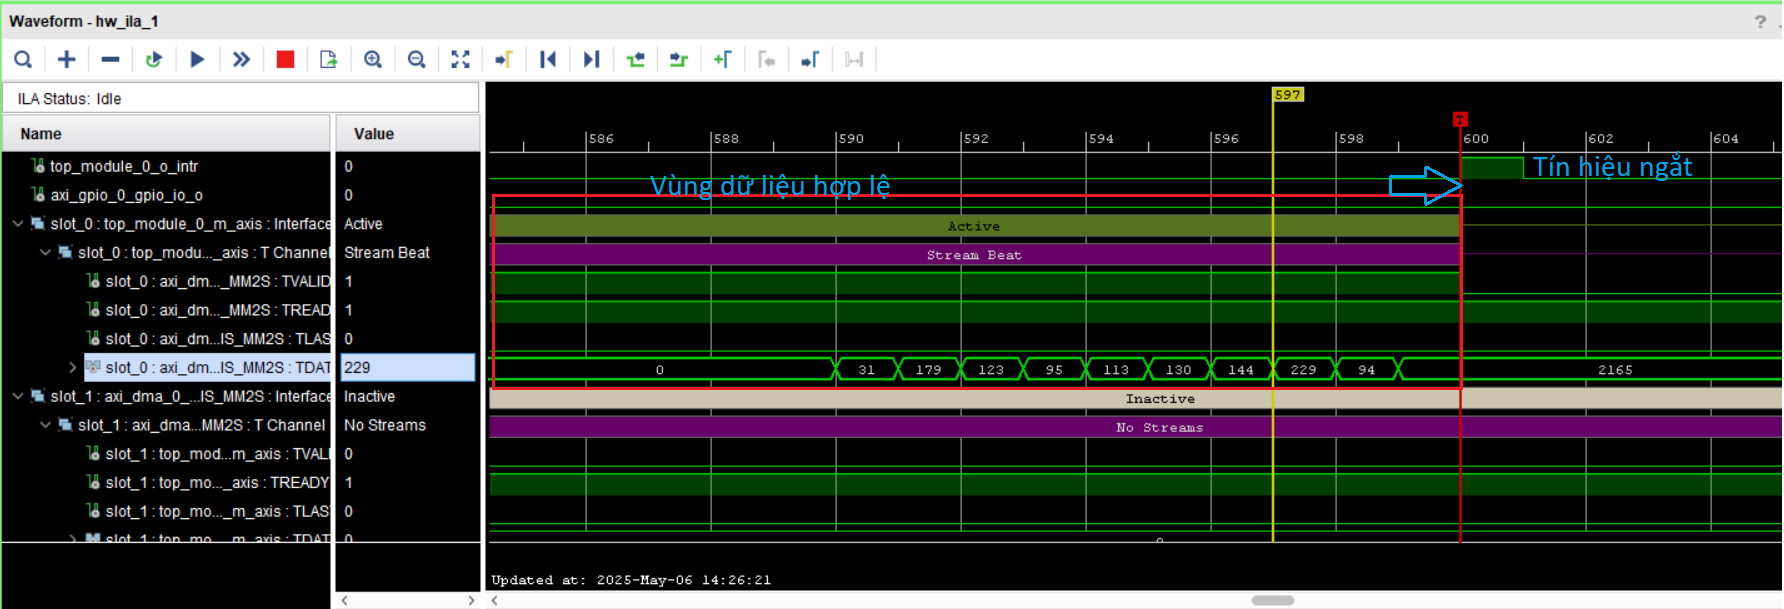
\includegraphics[width=\linewidth]{figures/ila1.png}
	\caption{ILA với điểm kích hoạt là \textit{o\_intr}}
	\label{fig:ila1}
\end{figure}
\begin{figure}[H]
	\centering
	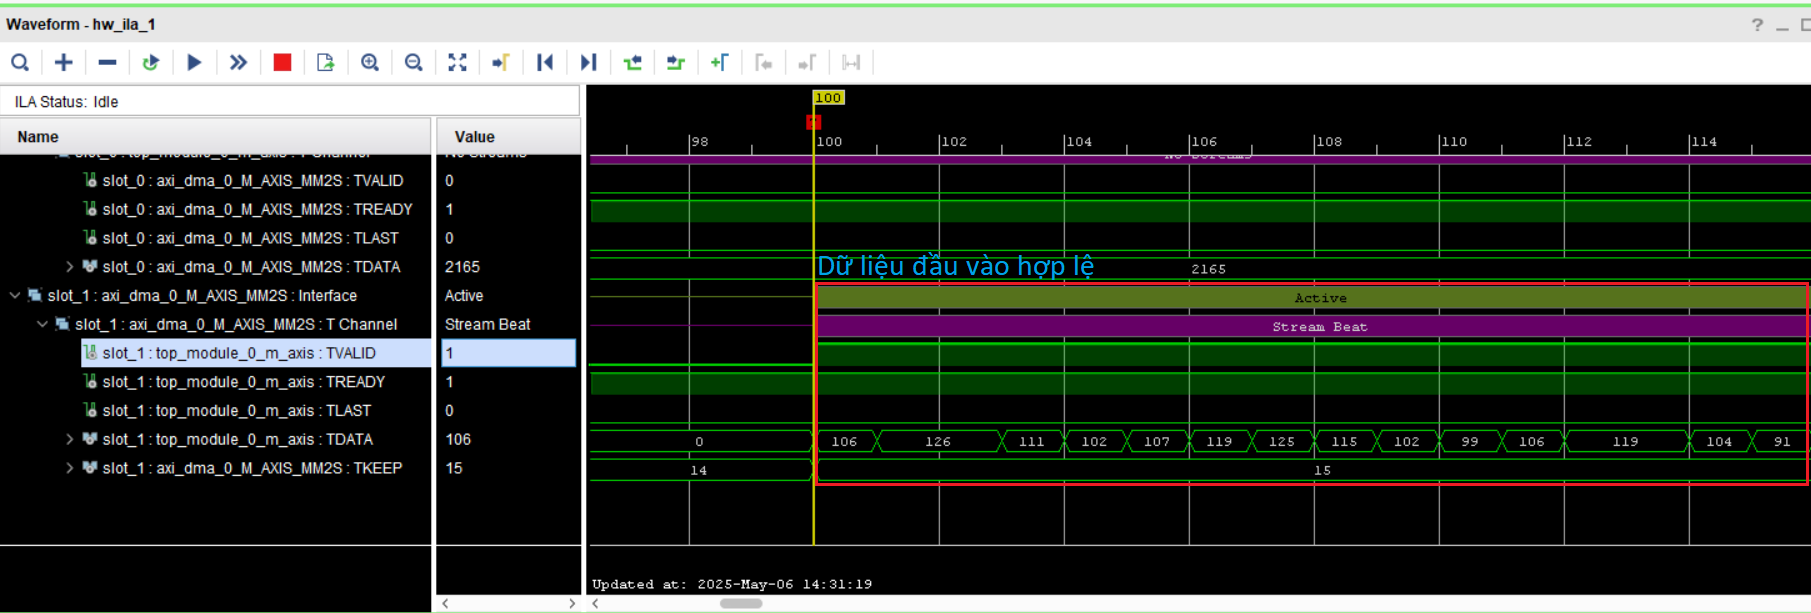
\includegraphics[width=\linewidth]{figures/ila3.png}
	\caption{ILA với dữ liệu điểm ảnh đầu vào}
	\label{fig:ila3}
\end{figure}


Để giám sát hoạt động của hệ thống sau khi triển khai, một IP được sử dụng trong thiết kế là Integrated Logic Analyzer (ILA). Kết quả thu được tương ứng với các hình \ref{fig:ila1}, \ref{fig:ila3}. Hình \ref{fig:ila1} cho thấy sau ngay sau khi nhận xong toàn bộ dữ liệu, tín hiệu ngắt được kích hoạt lên mức cao trong 1 chu kỳ, đảm bảo vi xử lý có thể xử lý được dữ liệu ngay khi hoàn tất quá trình tính toán.
